\documentclass[conference]{IEEEtran}

\usepackage[section]{placeins}
\usepackage[utf8]{inputenc}
\usepackage[T1]{fontenc}
\usepackage{cite}
\usepackage{hyperref}
\usepackage{url}
\usepackage{booktabs}
\usepackage{amsfonts}
\usepackage{microtype}
\usepackage{graphicx}
\hypersetup{hidelinks}
% This checks both possible locations for the uploaded figures.
\graphicspath{{figures/}{Figures/figures/}{highstakes/figures/}{highstakes/}}

\title{Decomposing Cross-Dataset Generalization Gaps in 12-Lead ECG Classification}

% AI4BioSig uses double-blind review. Keep author and affiliation fields empty.
\author{}

\begin{document}

\maketitle

\begin{abstract}
Deep learning models for automated ECG interpretation are typically trained and evaluated on a single dataset, and their performance can decline when applied to data collected elsewhere. We built a benchmark that trains and tests four architectures (InceptionTime, ResNet1D, a Transformer baseline, and the ECG-FM foundation model) across five public 12-lead ECG datasets: PTB-XL, CPSC2018, Georgia, MIMIC-IV-ECG, and CODE-15\%. ECG-FM achieved the highest mean in-distribution macro-AUROC (0.972). ResNet1D achieved the highest mean cross-dataset macro-AUROC (0.924) and the smallest generalization gap (0.042). Robustness depended strongly on transfer direction and endpoint definition. Matched-record normal-versus-abnormal evaluation reduced the pooled gap from 0.049 to 0.038 (22.5\%). Pairwise analysis showed that the mean gap fell for 10 of the 20 directional dataset pairs and grew for the other 10. Alternative endpoint mappings changed absolute AUROC; the model ranking remained the same. ECG-FM's lowest source-to-MIMIC-IV-ECG scores came mainly from normal and first-degree atrioventricular block. These findings place source-target direction and label harmonization at the center of the benchmark. Population and device differences provide supporting context.
\end{abstract}

\section{Introduction}

Deep learning models may match or outperform the performance of experts in 12-lead electrocardiogram (ECG) classification tasks using the same 12-lead ECG data for training and validation \cite{ribeiro2020}. However, this does not guarantee generalization across hospitals or datasets due to possible changes in the demographic structure, prevalence, and measurement process of the target disease \cite{subbaswamy2020}. Furthermore, several cross-dataset ECG studies have reported a drop in model performance when the training and evaluation sets differ \cite{wantlin2023}. In this paper, we identify and separate the sources of such changes into population, acquisition, and label-schema shifts.

These shifts might be related to each other; however, they cannot be addressed by similar solutions. While population shift might be mitigated through recalibration or prevalence-aware evaluation, acquisition shift can be solved by waveform normalization or augmentation. None of them can solve the inconsistency in diagnostic vocabularies, which should be handled separately by either explicit harmonization or new annotation. As such, combining them into a single distribution shift value hides the information needed to determine the appropriate action \cite{subbaswamy2020}. It is also not suitable for evaluating performance due to possible diversity in combinations of population, acquisition, and labeling differences that might lead to the same performance gap.

Labeling schema is particularly prone to being unnoticed because harmonization is considered as preprocessing and not a part of benchmark definition. For instance, PhysioNet Challenge documents list complete right bundle branch block and right bundle branch block as separate SNOMED-CT codes, 713427006 and 59118001, respectively \cite{alday2020}. Any harmonization that ignores the distinction can potentially reduce or even remove the corresponding class in the source dataset. In the same way, the PTB-XL database distinguishes between the rhythm statement of sinus rhythm, found in 16,782 samples, and the diagnostic statement of normal ECG, found in 9,528 samples \cite{wagner2020}. Although they describe the same thing conceptually, they are not interchangeable. In case the harmonization is not well-documented or documented at all, two studies using the same datasets can measure different generalization gaps as a result of different benchmark definitions.

This work introduces a cross-dataset generalization benchmark for 12-lead ECG classification based on PTB-XL, CPSC2018, the Georgia 12-lead Challenge database, MIMIC-IV-ECG, and CODE-15\% \cite{wagner2020,alday2020,gow2023,code15}. Every recording follows a common signal contract, and source-specific diagnoses are mapped to five shared endpoints. We train four model families on each available source and evaluate every trained model on all five targets. The design produces 25 directional evaluations per architecture and 100 evaluations overall. For each off-diagonal transfer, we record population, acquisition, and labeling differences. We also use normal-versus-abnormal and alternative-mapping analyses to test how the endpoint definition affects the findings. This view of the benchmark reveals changes in model ranking, strong directional effects, and sensitivity to label granularity that a within-dataset score would miss.

The main contribution is a benchmark that shows how cross-dataset ECG robustness changes with transfer direction and diagnostic-label harmonization. Its five open-source datasets span four continents: PTB-XL from Germany, CPSC2018 from China, Georgia and MIMIC-IV-ECG from the United States, and CODE-15\% from Brazil \cite{wagner2020,alday2020,gow2023,code15}. We record population and device differences for every ordered pair. Because those differences occur together in this observational setting, we use them to describe each transfer and avoid causal claims.

This work makes four contributions. First, we release the complete label mapping as a versioned, citable artifact, in which every source code carries a rule identifier, every exclusion has a written rationale, and ambiguous codes record their rejected alternatives, so the mapping can be audited rather than taken on faith. Second, we show that the diagnostic classes expressible across all four schemas represented in this benchmark form a strict set intersection of exactly five members, and we document what information is lost at its boundaries. Third, we provide a protocol that isolates the three shift components instead of collapsing them into a single aggregate gap, reporting the attribution alongside a sensitivity analysis rather than as fixed ground truth. Fourth, we quantify label-schema sensitivity through matched-record normal-versus-abnormal evaluation and three alternative endpoint mappings.

The datasets are available through public repositories, subject to their individual access requirements. The released pipeline documents the preprocessing, training, evaluation, and sensitivity-analysis steps required to reproduce the benchmark.

\section{Related Works}

Public ECG benchmarking currently focuses on within-dataset evaluation, and the datasets themselves are the source of the label-schema problem that our benchmark measures. PTB-XL utilized the SCP-ECG coding standard for its 21,000+ recordings \cite{wagner2020}, whilst other datasets like CPSC2018 and the Georgia 12-lead database exist under the SNOMED-CT schema \cite{alday2020}. These schemas were independently defined and were not designed to be comparable with one another, leading to scenarios where the same diagnosis may have different coding standards. This is why a unified five-class mapping across four coding systems is more complex than it lets on.

When cross-dataset evaluation has occurred, a performance drop can occur, yet no diagnosis has been given as to why such events occur. This is particularly relevant in the case of Cardioformer, which performed excellently when trained and tested on MIMIC-IV, achieving a 96.3\% AUROC; however, when that same trained model was evaluated on PTB, the accuracy plummeted to 49.2\% AUROC \cite{mobin2025}. The closest prior attempt at identifying this gap is BenchMD, which constructs a cross-dataset ECG evaluation using PTB-XL as a training source against Chapman-Shaoxing, Georgia, and CPSC2018 as targets, and explicitly mentions demographic and device-collection differences as the source behind the accuracy gap \cite{wantlin2023}. BenchMD does mention categories that contribute to this gap, yet fails to quantify the extent to which these categories contribute. Additionally, it fails to consider label-schema shift despite pairing datasets with incompatible native coding systems. This project extends BenchMD's categories into the analytical core of a benchmark, a directional train/test matrix with per-cell shift attribution, rather than simply a qualitative observation.

A recent position paper argues that current ECG representation benchmarks can produce misleading comparisons. Berger et al. found that, under several common evaluation settings, a randomly initialized encoder with linear evaluation could match state-of-the-art pretrained representations \cite{berger2026}. Their concern is complementary to ours: they question what existing benchmarks reward, whereas our study asks what changes when the training and evaluation sources diverge.

Foundation models also complicate the meaning of held-out evaluation. ECG-FM was pretrained on MIMIC-IV-ECG and the PhysioNet Challenge 2021 collection \cite{mckeen2025}. The latter contains PTB-XL, CPSC2018, and Georgia \cite{reyna2021}, so four of the five datasets in our benchmark overlap with ECG-FM's pretraining sources. We therefore interpret its results as performance after broad pretraining exposure rather than as fully independent evaluation. This distinction lets us examine whether prior exposure is enough to prevent the directional generalization failures observed in the benchmark.

No existing work pairs the five major public 12-lead ECG datasets in a directional train/test matrix with each cross-dataset cell attributed to a specific, quantified combination of population, device, and label-schema shift. That is this project's contribution.

\section{Methods}

\begin{figure*}[!t]
    \centering
    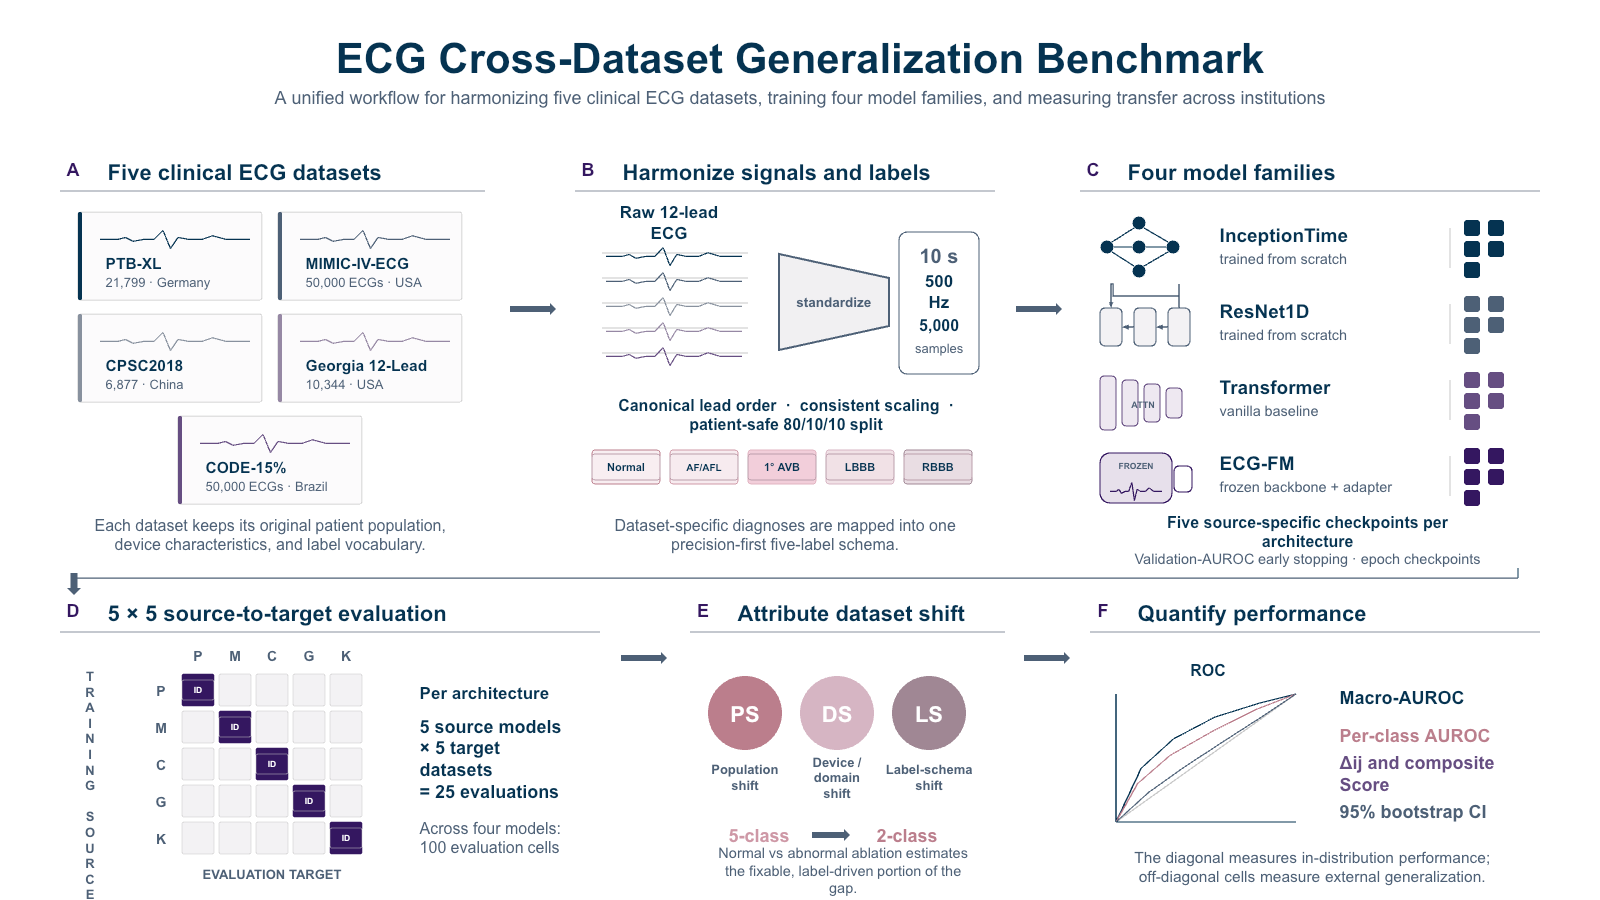
\includegraphics[width=\textwidth,height=0.34\textheight,keepaspectratio]{fig1_methods_pipeline.png}
    \caption{Construction and evaluation of the cross-dataset benchmark. \textbf{A}, five public 12-lead ECG datasets retain their original patient populations, acquisition conditions, and diagnostic vocabularies. \textbf{B}, waveforms are placed on a common signal contract with a canonical lead order, consistent scaling, and 10 seconds at 500 Hz (5,000 samples). Records are split by patient where identifiers permit. Source diagnoses are mapped to normal sinus rhythm, atrial fibrillation or flutter (AF/AFL), first-degree atrioventricular block (1$^{\circ}$ AVB), left bundle branch block (LBBB), and right bundle branch block (RBBB). \textbf{C}, InceptionTime, ResNet1D, and the Transformer are trained from scratch. ECG-FM uses a frozen pretrained backbone with a study-specific adapter. Validation AUROC selects five source-specific checkpoints for each architecture. \textbf{D}, every source model is evaluated on all five targets. Each architecture produces a $5\times5$ matrix, giving 25 cells per model family and 100 evaluations overall. Diagonal cells are in-distribution tests; off-diagonal cells measure external transfer. \textbf{E}, each ordered source-target pair is described by population (PS), device or domain (DS), and label-schema (LS) indicators. A post-hoc normal-versus-abnormal analysis supplements the five-class analysis. \textbf{F}, reported outcomes include macro-AUROC, per-class AUROC, the in-distribution-to-external generalization gap, a descriptive composite score for sensitivity analysis, and prediction-level 95\% bootstrap confidence intervals.}
    \label{fig:methods-pipeline}
\end{figure*}

\paragraph{Datasets.} We use PTB-XL (21,837 records, Germany), a 50,000-record subsample of MIMIC-IV-ECG (United States), the Georgia 12-lead ECG Challenge database (10,344 records, United States), CPSC2018 (6,877 records, China), and a 50,000-record stratified subsample of CODE-15\% (Brazil). Together, these sources span four distinct labeling schemas: SCP-ECG statements, SNOMED-CT concept identifiers, a nine-class integer scheme, and a six-label boolean scheme.

\paragraph{Label harmonization.} Because CPSC2018 and CODE-15\% rely on closed vocabularies, the set of classes natively representable across all sources is their intersection, which yields five members: normal sinus rhythm, atrial fibrillation or flutter, first-degree atrioventricular block, left bundle branch block, and right bundle branch block. We map every source code to these classes using an explicit rule typology distinguishing direct assignment, merge, proxy, and derivation. Normal sinus rhythm is provided in two variants, one defined as sinus rhythm and the other as normal ECG, as no single definition is native to all schemas. The complete mapping, including its exclusions and unresolved ambiguities, is released alongside this work.

\paragraph{Models and splits.} We evaluate InceptionTime, ResNet1D, a vanilla Transformer, and ECG-FM on the harmonized five-class multi-label task. The first three architectures are trained from scratch, whereas ECG-FM uses its pretrained backbone with the study-specific adapter. Splits are constructed at the patient level where identifiers permit, stratified on the rarest class rather than drawn at random, and constrained to guarantee a minimum number of positive examples per class per evaluation fold. MIMIC-IV-ECG and CODE-15\% are subsampled with stratification rather than uniformly so as to preserve their class composition.

\paragraph{Evaluation.} We report macro-AUROC and per-class AUROC for each source-to-target evaluation. Population, device, and label-schema indicators are recorded for every ordered dataset pair. The composite shift score appears only in a sensitivity analysis because its weights reflect analytic choices. The revision analyses use the saved five-class predictions and do not retrain the models. For the normal-versus-abnormal analysis, we combine the four abnormal-class probabilities and evaluate the same eligible records used in the five-class task. The mapping sensitivity analysis tests an exclusive definition of normal, a task that removes the ambiguous normal class, and a task that combines LBBB with RBBB.

\paragraph{Directional and MIMIC-IV-ECG audits.} We recomputed the generalization gap for all 80 off-diagonal architecture-source-target cells using records eligible for both the five-class and normal-versus-abnormal tasks. The signed change equals the matched five-class gap minus the binary gap. We then averaged that change across the four architectures for each of the 20 ordered dataset pairs. A positive value means the binary endpoint reduced the gap. For every ECG-FM source-to-MIMIC-IV-ECG cell, we also compare training-label prevalence, available acquisition metadata, and per-class AUROC. Model-level hardware information was unavailable for CPSC2018, Georgia, and MIMIC-IV-ECG. The audit is therefore descriptive and cannot isolate a device effect.

\section{Results}

Table~\ref{tab:model-summary} and Figure~\ref{fig:generalization}A summarize performance by architecture. Figure~\ref{fig:heatmaps} shows all 100 source-to-target evaluations. The model ranking changes between internal and external evaluation. ECG-FM had the highest mean in-distribution macro-AUROC (0.972), followed by ResNet1D (0.966), InceptionTime (0.965), and the Transformer (0.937). Across datasets, ResNet1D moved to first place with a mean macro-AUROC of 0.924 and the smallest generalization gap (0.042). InceptionTime followed at 0.919 with a gap of 0.046. ECG-FM reached 0.888 with a gap of 0.085, and the Transformer reached 0.879 with a gap of 0.058. Selecting a model from its in-distribution score alone would therefore have chosen the architecture with the largest average external-performance loss.

\begin{table}[!htbp]
    \caption{Mean five-class macro-AUROC across the five in-distribution cells and 20 cross-dataset cells for each architecture. The generalization gap is the difference between the two means.}
    \label{tab:model-summary}
    \centering
    \small
    \begin{tabular}{lccc}
        \toprule
        Model & In-distribution & Cross-dataset & Gap \\
        \midrule
        ResNet1D      & 0.966 & \textbf{0.924} & \textbf{0.042} \\
        InceptionTime & 0.965 & 0.919 & 0.046 \\
        ECG-FM        & \textbf{0.972} & 0.888 & 0.085 \\
        Transformer   & 0.937 & 0.879 & 0.058 \\
        \bottomrule
    \end{tabular}
\end{table}

\begin{figure*}[!t]
    \centering
    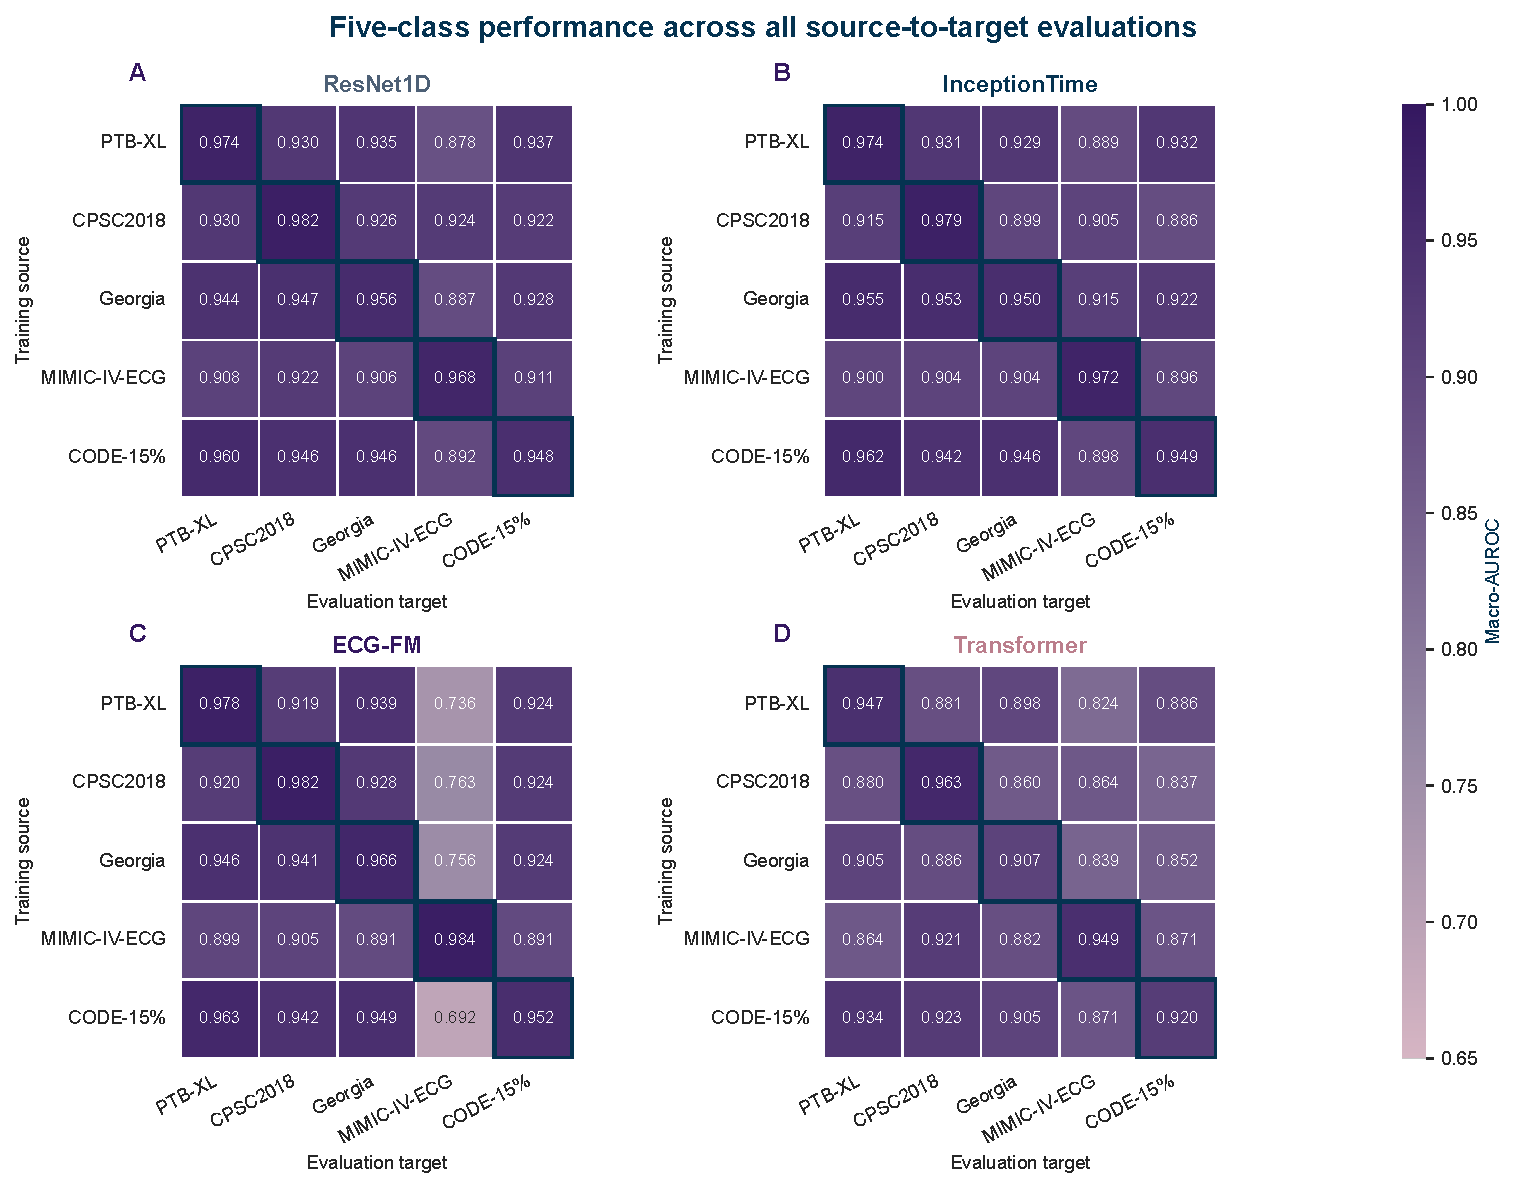
\includegraphics[width=\textwidth,height=0.42\textheight,keepaspectratio]{fig2_four_model_heatmaps.pdf}
    \caption{Five-class macro-AUROC for all 100 source-to-target evaluations. Rows denote the training source and columns denote the evaluation target; outlined diagonal cells are in-distribution evaluations. All panels share one color scale. The variation across off-diagonal cells, including the consistently difficult MIMIC-IV-ECG target and several asymmetric source-target pairs, shows why one aggregate score cannot describe cross-dataset behavior.}
    \label{fig:heatmaps}
\end{figure*}

The full matrices show that transfer difficulty depends on the target and the direction of evaluation (Figure~\ref{fig:heatmaps}). Averaged across external sources and architectures, MIMIC-IV-ECG was the hardest target, with a macro-AUROC of 0.846. The corresponding averages were 0.903 for CODE-15\%, 0.915 for Georgia, 0.924 for PTB-XL, and 0.925 for CPSC2018 (Figure~\ref{fig:generalization}B). Direction mattered as well. Transfer from MIMIC-IV-ECG to PTB-XL averaged 0.892 across the four architectures; PTB-XL to MIMIC-IV-ECG averaged 0.832. ECG-FM showed the largest single-model contrast. Its CODE-15\%-to-MIMIC-IV-ECG AUROC was 0.692, compared with 0.891 in the reverse direction. A dataset therefore has no fixed level of transfer difficulty. Its role as the source or target changes the result.

ECG-FM's results on MIMIC-IV-ECG make the same point at the model level. Its diagonal AUROC on MIMIC-IV-ECG was 0.984. When ECG-FM models trained on the other four sources were evaluated on MIMIC-IV-ECG, the mean fell to 0.737, a drop of 0.247. The corresponding drops were 0.070 for InceptionTime, 0.073 for ResNet1D, and 0.099 for the Transformer. ECG-FM had already seen MIMIC-IV-ECG during pretraining, so prior source exposure alone did not produce reliable transfer under the harmonized endpoint used here. The result cannot separate the effects of population, acquisition, and labeling differences.

Table~\ref{tab:mimic-audit} gives a more detailed view of the ECG-FM source-to-MIMIC result. The two lowest macro-AUROCs were CODE-15\%$\rightarrow$MIMIC-IV-ECG at 0.692 and PTB-XL$\rightarrow$MIMIC-IV-ECG at 0.736. Normal had AUROCs of 0.594 and 0.649 in those cells, and first-degree atrioventricular block had AUROCs of 0.623 and 0.619. LBBB remained between 0.795 and 0.808. Prevalence also varied sharply. Normal was positive in 80.9\% of the MIMIC-IV-ECG target records, compared with 38.3\% of the CODE-15\% training records and 43.6\% of the PTB-XL training records. CODE-15\% was recorded at 400~Hz and resampled to the 500~Hz benchmark contract. Hardware information is incomplete for several other sources. These class-specific results and metadata differences point to an endpoint- and source-dependent mismatch. The observational comparison does not establish which factor caused it.

\begin{table*}[!t]
    \caption{ECG-FM audit for each source evaluated on MIMIC-IV-ECG. Prevalence and AUROC vectors follow the order normal/AF--AFL/1$^{\circ}$ AVB/LBBB/RBBB. Prevalence is measured in each source training split; the MIMIC-IV-ECG row reports its training prevalence and diagonal test AUROC. A dash in hardware means the public metadata used here did not identify a model.}
    \label{tab:mimic-audit}
    \centering
    \scriptsize
    \resizebox{\textwidth}{!}{%
    \begin{tabular}{lclcc}
        \toprule
        Source & Native acquisition & Training prevalence (\%) & Per-class AUROC on MIMIC-IV-ECG & Macro \\
        \midrule
        PTB-XL      & 500 Hz; Schiller & 43.6/7.2/3.6/2.5/2.5  & .649/.884/.619/.795/.735 & .736 \\
        CPSC2018    & 500 Hz; --       & 13.3/17.8/10.5/3.4/27.0 & .720/.820/.693/.851/.729 & .763 \\
        Georgia     & 500 Hz; --       & 16.9/7.2/7.4/2.2/5.2  & .657/.853/.644/.834/.793 & .756 \\
        CODE-15\%   & 400 Hz; TEB/Micromed & 38.3/2.1/1.7/1.7/2.7 & .594/.702/.623/.808/.732 & .692 \\
        MIMIC-IV-ECG & 500 Hz; multi-vendor, models undisclosed & 80.9/11.9/7.4/3.7/8.2 & .986/.992/.984/.976/.979 & .984 \\
        \bottomrule
    \end{tabular}}
\end{table*}

\begin{figure}[!htbp]
    \centering
    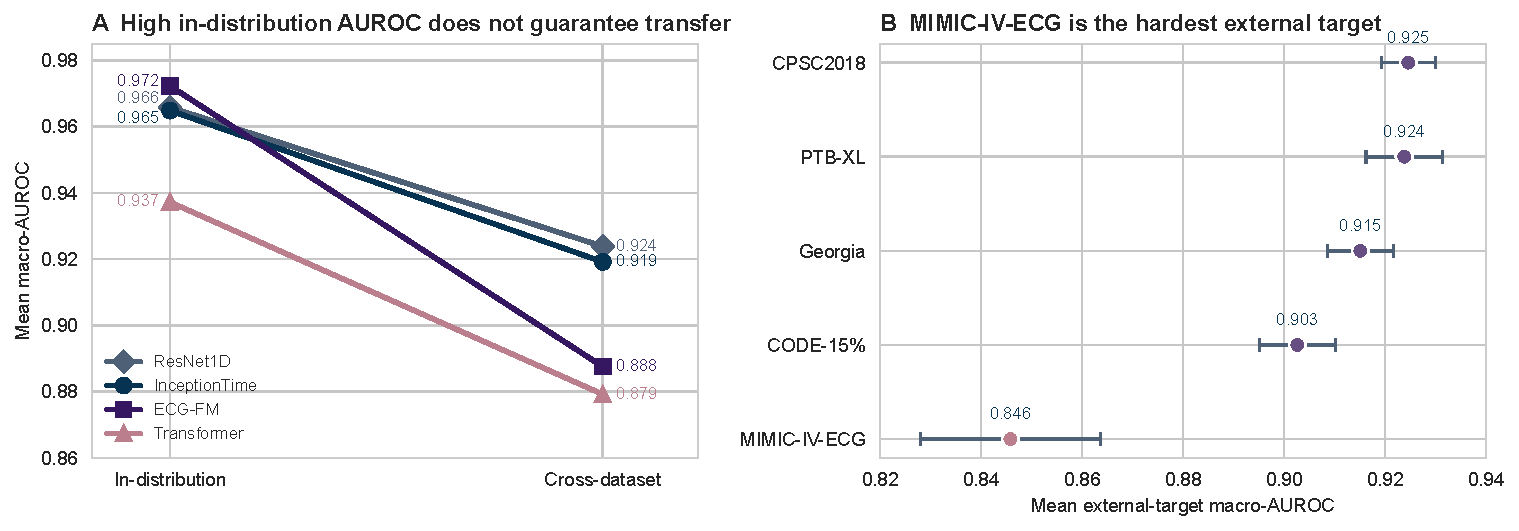
\includegraphics[width=\linewidth,height=0.40\textheight,keepaspectratio]{fig3_generalization_summary.pdf}
    \caption{Generalization summary. Panel A shows the change in model order between the two evaluation settings. ECG-FM leads on in-distribution data, and ResNet1D leads on external data. Panel B shows that MIMIC-IV-ECG is the hardest evaluation target after averaging across models and external sources. Error bars represent the standard error across the contributing source-model cells.}
    \label{fig:generalization}
\end{figure}

We grouped the off-diagonal cells using the population, device, and label-schema indicators introduced in Figure~\ref{fig:methods-pipeline}E. A one-way ANOVA across all four architectures ($n=80$) found no significant difference in raw gap magnitude among the observed shift-vector groups ($F=0.14$, $p=0.87$). This analysis offers no evidence that one shift category caused a fixed share of the performance loss. We use the weighted composite score only to examine sensitivity to the chosen weights. Raw cross-dataset AUROC and the unweighted generalization gap remain the primary results.

The post-hoc analyses show how much the benchmark endpoint affects the gap (Figure~\ref{fig:sensitivity}). Using the same eligible records, the normal-versus-abnormal task reduced the pooled average gap from 0.049 to 0.038, or 22.5\%. Pairwise results varied considerably. The gap decreased in 47 of the 80 architecture-specific off-diagonal cells and increased in 33. After averaging across architectures, 10 of the 20 ordered dataset pairs improved and 10 worsened (Table~\ref{tab:binary-pairs}). The largest reductions occurred when MIMIC-IV-ECG was the source, ranging from 6.59 to 8.67 percentage points across its four external targets. CPSC2018$\rightarrow$MIMIC-IV-ECG showed the largest increase, with a binary gap 6.95 points larger. Label simplification changes where the benchmark appears difficult, and its effect is far from uniform.

\begin{table}[!t]
    \caption{Change in the matched-record generalization gap after collapsing five labels to normal versus abnormal, averaged over four architectures, in percentage points. Rows are training sources and columns are evaluation targets. Positive values mean the binary endpoint reduced the gap; negative values mean it increased the gap.}
    \label{tab:binary-pairs}
    \centering
    \small
    \resizebox{\columnwidth}{!}{%
    \begin{tabular}{lrrrrr}
        \toprule
        Source $\backslash$ Target & PTB-XL & CPSC2018 & Georgia & MIMIC-IV & CODE-15\% \\
        \midrule
        PTB-XL      & --    & +2.99 & +2.44 & +0.46 & +0.45 \\
        CPSC2018    & -1.04 & --    & -1.16 & -6.95 & -0.26 \\
        Georgia     & -1.86 & -0.11 & --    & -3.99 & -1.39 \\
        MIMIC-IV-ECG & +6.59 & +8.31 & +6.62 & --    & +8.67 \\
        CODE-15\%   & -0.01 & +0.96 & +1.93 & -0.65 & -- \\
        \bottomrule
    \end{tabular}}
\end{table}

At the architecture level, the gap fell by 1.8\% for ECG-FM, 41.8\% for InceptionTime, 43.7\% for ResNet1D, and 24.8\% for the Transformer (Figure~\ref{fig:sensitivity}A). The controlled endpoint analysis used the same saved predictions and eligible records under three alternative definitions. One rule made normal exclusive, one removed the normal endpoint, and one merged LBBB with RBBB. Mean cross-dataset macro-AUROC was 0.902 for the consensus five-class mapping. The three alternatives produced values of 0.902, 0.932, and 0.887. All four mappings kept the same model order: ResNet1D, InceptionTime, ECG-FM, and Transformer (Figure~\ref{fig:sensitivity}B). These analyses use fixed predictions and measure sensitivity to endpoint definition.

\begin{figure}[!htbp]
    \centering
    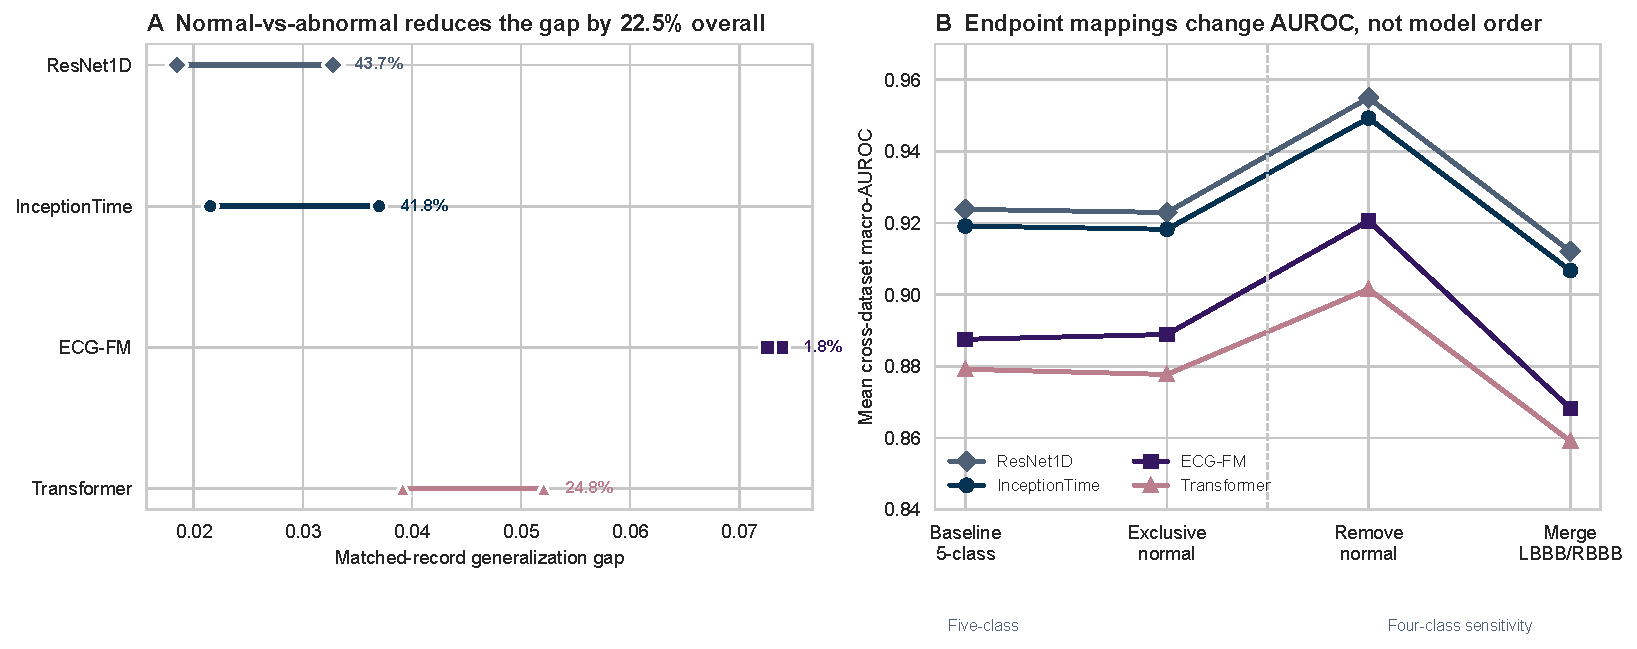
\includegraphics[width=\linewidth,height=0.40\textheight,keepaspectratio]{fig4_revision_sensitivity.pdf}
    \caption{Post-hoc sensitivity analyses using fixed saved predictions. Panel A shows the change in the matched-record generalization gap under normal-versus-abnormal evaluation, with results reported separately for each architecture. Panel B shows absolute macro-AUROC under each alternative endpoint mapping; the model order remains unchanged. The four-class variants serve as sensitivity diagnostics and should be interpreted on their own task definitions.}
    \label{fig:sensitivity}
\end{figure}

\FloatBarrier
\section{Discussion}

The clearest finding is the change in model ranking between internal and external evaluation. ECG-FM led the in-distribution comparison with a macro-AUROC of 0.972. Its mean cross-dataset AUROC fell to 0.888, producing a gap of 0.085. ResNet1D began with a slightly lower in-distribution AUROC of 0.966 and reached the best external mean at 0.924, with a gap of 0.042 (Table~\ref{tab:model-summary}; Figure~\ref{fig:generalization}A). In this comparison, the best internal score belonged to the model with the largest average loss on external data. The diagonal of a benchmark matrix cannot substitute for external validation.

The source-target matrices also show that generalization is directional. Across architectures, MIMIC-IV-ECG to PTB-XL averaged 0.892; PTB-XL to MIMIC-IV-ECG averaged 0.832. ECG-FM produced a larger asymmetry between CODE-15\% and MIMIC-IV-ECG, with 0.692 in the CODE-15\%-to-MIMIC-IV-ECG direction and 0.891 in the reverse direction (Figure~\ref{fig:heatmaps}). These examples show why a pair of datasets cannot be described by a single notion of closeness. The source shapes what the model learns. The target determines the population, signal characteristics, and labels encountered during evaluation. The same pair can therefore be easy in one direction and difficult in the other.

MIMIC-IV-ECG provides a concrete example of target-specific difficulty. Its pooled external-target AUROC was 0.846, the lowest among the five datasets (Figure~\ref{fig:generalization}B). ECG-FM scored 0.984 on the MIMIC-IV-ECG diagonal. Models trained on the other four sources averaged 0.737 when evaluated on MIMIC-IV-ECG. Table~\ref{tab:mimic-audit} shows that the largest and most consistent losses occurred in normal and first-degree atrioventricular block. Training-label prevalences differed substantially from those in MIMIC-IV-ECG, and acquisition hardware was incompletely documented. ECG-FM had seen MIMIC-IV-ECG and three other benchmark sources during pretraining. Even with that exposure, mismatch remained at the downstream endpoint. The available evidence cannot determine whether population, acquisition, labeling, or a combination of them produced the loss.

The endpoint analyses offer more direct evidence that label definition contributes to the measured gap. The design remains non-causal. The pooled gap fell by 22.5\%. At the pair level, the gap decreased for half of the directional pairs and increased for the other half (Table~\ref{tab:binary-pairs}). The reduction ranged from 1.8\% for ECG-FM to 43.7\% for ResNet1D (Figure~\ref{fig:sensitivity}A). Label granularity changes some apparent failures, and its effect varies across transfers. Removing the ambiguous normal endpoint increased mean cross-dataset macro-AUROC to 0.932. Merging LBBB with RBBB reduced it to 0.887. Neither change altered the model ranking (Figure~\ref{fig:sensitivity}B). In this experiment, task construction had a larger effect on absolute scores than on the ordering of the architectures.

The shift indicators provide a structured description of each transfer. They do not provide a causal decomposition. Population, device, and label-schema differences co-occur in most transfers, and the raw gaps did not differ significantly across the observed shift-vector groups ($F=0.14$, $p=0.87$). The evidence does not support assigning a fixed percentage of the loss to label schema or any other component. The benchmark makes these assumptions visible, reports the raw directional cells, and checks whether the conclusions hold under reasonable endpoint changes. The ranking change, directional asymmetries, difficult MIMIC-IV-ECG target, and stable model order under the mapping analysis all lead to the same practical recommendation. ECG models should be compared on several external targets, and each benchmark should report the exact label mapping and source-to-target matrix behind its aggregate scores.

\FloatBarrier
\section{Limitations}

The benchmark covers five diagnostic classes, leaving other abnormalities in the original datasets outside its scope. Mapping different coding systems into the same classes requires judgment, and different defensible choices may change the absolute results. Population, device, and label-schema indicators also co-occur, while acquisition hardware is incompletely documented for three datasets. Subsampling MIMIC-IV-ECG and CODE-15\% may omit rare patterns. Finally, retrospective AUROC does not directly measure calibration, fairness, clinical safety, or real-world patient outcomes.

\section{Conclusion}

This study shows that strong performance within one ECG dataset does not guarantee robust performance on data collected elsewhere. Robustness changed with source-target direction and with the way diagnostic labels were harmonized. ECG-FM had the highest mean in-distribution AUROC. ResNet1D had the highest cross-dataset AUROC and the smallest gap. MIMIC-IV-ECG was the most difficult external target, with ECG-FM losses concentrated in specific classes and accompanied by large prevalence differences and incomplete acquisition metadata. The normal-versus-abnormal endpoint reduced the pooled gap. Half of the directional pairs improved. Alternative endpoint mappings changed absolute scores, and the model order stayed the same. Population and device indicators help describe these results. The observational design does not support causal attribution. A useful ECG benchmark should report the full directional matrix, per-class behavior, and exact label mapping alongside any pooled score.

\section{Responsible Use Statement}

This benchmark is intended for research use and should not be interpreted as evidence that any evaluated model is ready for clinical deployment. The reported results measure cross-dataset performance on retrospective ECG datasets rather than real-world clinical safety. Model rankings may also depend on label harmonization and benchmark design choices. Therefore, these results should be used to study model robustness rather than guide patient diagnosis or treatment. Clinical use would require additional validation on representative patient populations under real-world conditions.

\begin{thebibliography}{11}

\bibitem{berger2026}
Berger, Z., Prakah-Asante, D., Guttag, J., \& Stultz, C.M. (2026).
Position: Evaluation of ECG representations must be fixed.
\textit{arXiv preprint arXiv:2602.17531}.

\bibitem{gow2023}
Gow, B., Pollard, T., Nathanson, L.A., Johnson, A., Moody, B., Fernandes, C., Greenbaum, N., Waks, J.W., Eslami, P., Carbonati, T., Chaudhari, A., Herbst, E., Moukheiber, D., Berkowitz, S., Mark, R., \& Horng, S. (2023).
MIMIC-IV-ECG: Diagnostic Electrocardiogram Matched Subset (version 1.0).
\textit{PhysioNet}. \url{https://doi.org/10.13026/4nqg-sb35}.

\bibitem{mckeen2025}
McKeen, K., Masood, S., Toma, A., Rubin, B., \& Wang, B. (2025).
ECG-FM: an open electrocardiogram foundation model.
\textit{JAMIA Open}, 8(5), ooaf122.

\bibitem{mobin2025}
Mobin, M.K., Islam, M.S., Barid, S.A., \& Masum, M. (2025).
Cardioformer: Advancing AI in ECG analysis with multi-granularity patching and ResNet.
\textit{arXiv preprint arXiv:2505.05538}.

\bibitem{alday2020}
Perez Alday, E.A., Gu, A., Shah, A.J., Robichaux, C., Wong, A.K.I., Liu, C., Liu, F., Rad, A.B., Elola, A., Seyedi, S., Li, Q., Sharma, A., Clifford, G.D., \& Reyna, M.A. (2020).
Classification of 12-lead ECGs: the PhysioNet/Computing in Cardiology Challenge 2020.
\textit{Physiological Measurement}, 41(12), 124003.

\bibitem{reyna2021}
Reyna, M.A., Sadr, N., Perez Alday, E.A., Gu, A., Shah, A.J., Robichaux, C., Rad, A.B., Elola, A., Seyedi, S., Ansari, S., Ghanbari, H., Li, Q., Sharma, A., \& Clifford, G.D. (2021).
Will two do? Varying dimensions in electrocardiography: the PhysioNet/Computing in Cardiology Challenge 2021.
In \textit{2021 Computing in Cardiology}, 1--4.

\bibitem{ribeiro2020}
Ribeiro, A.H., Ribeiro, M.H., Paix\~{a}o, G.M.M., Oliveira, D.M., Gomes, P.R., Canazart, J.A., Ferreira, M.P.S., Andersson, C.R., Macfarlane, P.W., Meira, W. Jr., Sch\"{o}n, T.B., \& Ribeiro, A.L.P. (2020).
Automatic diagnosis of the 12-lead ECG using a deep neural network.
\textit{Nature Communications}, 11, 1760.

\bibitem{code15}
Ribeiro, A.H., Paix\~{a}o, G.M.M., Lima, E.M., Ribeiro, M.H., Pinto Filho, M.M., Gomes, P.R., Oliveira, D.M., Meira, W. Jr., Sch\"{o}n, T.B., \& Ribeiro, A.L.P. (2021).
CODE-15\%: a large scale annotated dataset of 12-lead ECGs.
\textit{Zenodo}. \url{https://doi.org/10.5281/zenodo.4916206}.

\bibitem{subbaswamy2020}
Subbaswamy, A., \& Saria, S. (2020).
From development to deployment: dataset shift, causality, and shift-stable models in health AI.
\textit{Biostatistics}, 21(2), 345--352.

\bibitem{wagner2020}
Wagner, P., Strodthoff, N., Bousseljot, R.D., Kreiseler, D., Lunze, F.I., Samek, W., \& Schaeffter, T. (2020).
PTB-XL, a large publicly available electrocardiography dataset.
\textit{Scientific Data}, 7(1), 154.

\bibitem{wantlin2023}
Wantlin, K., Wu, C., Huang, S.-C., Banerjee, O., Dadabhoy, F., Mehta, V.V., Han, R.W., Cao, F., Narayan, R.R., Colak, E., Adamson, A., Heacock, L., Tison, G.H., Tamkin, A., \& Rajpurkar, P. (2023).
BenchMD: A benchmark for unified learning on medical images and sensors.
\textit{arXiv preprint arXiv:2304.08486}.

\end{thebibliography}

\end{document}
